% ============================================================
%  Modul 4 — Automasi dengan Bash Scripting
% ============================================================

\chapter{Automasi Bash Scripting}
\label{chap:modul-04}

% --- 1. Tujuan dan Output Praktikum ---
\section{Tujuan dan Output Praktikum}

\subsection{Tujuan Praktikum}
Setelah menyelesaikan praktikum ini, mahasiswa diharapkan mampu:
\begin{enumerate}
	\item Menjelaskan konsep dasar \textit{shell scripting} dan perannya dalam proses automasi sistem operasi.
	\item Memahami sintaks dasar skrip \textit{bash}, termasuk pemanfaatan variabel dan deklarasi \textit{shebang}.
	\item Membuat \textit{Shell Script} (.sh) sederhana dengan menggabungkan perintah-perintah dasar sistem file Linux seperti \texttt{mkdir}, \texttt{cp}, dan \texttt{cat} \cite{shotts2019linux}.
	\item Memberikan dan mengeksekusi hak akses (\textit{execute permissions}) pada skrip agar dapat dijalankan secara legal oleh sistem operasi.
\end{enumerate}

\subsection{Output Praktikum}
Pada akhir praktikum ini, mahasiswa diharapkan menghasilkan:
\begin{itemize}
	\item File \textit{shell script} berekstensi \texttt{.sh} yang memuat rangkaian instruksi automasi \textit{backup}.
	\item Direktori cadangan (\textit{backup}) yang tercipta secara otomatis dari hasil eksekusi skrip tersebut.
	\item Dokumentasi verifikasi keberhasilan pemberian izin status \textit{executable} pada file skrip.
\end{itemize}

% --- 2. Dasar Teori ---
\newpage
\section{Dasar Teori}

\subsection{Pengantar Automasi dan Bash Scripting}
\textit{Shell Scripting} adalah proses penggabungan serangkaian instruksi baris perintah (CLI) ke dalam sebuah teks file murni yang nantinya akan dieksekusi secara otomatis oleh penerjemah sistem (\textit{shell}). Pada Linux, setiap perintah dieksekusi melalui shell, yaitu program yang menyediakan lingkungan kerja bagi pengguna untuk berinteraksi dengan sistem operasi \cite{robbins2005classic}. 

Secara analogi, bayangkan sistem operasi Linux Anda sebagai seorang koki. Mengetik perintah satu per satu di terminal ibarat Anda berdiri di dapur dan mendiktekan instruksi memasak kalimat demi kalimat. Hal ini efisien untuk masakan sederhana, namun melelahkan untuk tugas rumit. Sebaliknya, \textit{Shell Scripting} ibarat Anda menyusun "Resep Masakan" utuh di secarik kertas, di mana instruksi seperti menyalin file (\texttt{cp}) atau memindahkan direktori (\texttt{mv}) dapat dijalankan secara mandiri dan konsisten dari awal hingga selesai \cite{das2012unix}.

\subsection{Struktur Skrip: Shebang dan Variabel}
Sebuah \textit{shell script} yang terstandarisasi selalu diawali dengan rangkaian karakter khusus yang disebut \textbf{Shebang} (\texttt{\#!/bin/bash}). Baris pertama ini adalah pengarah yang memberitahu \textit{kernel} sistem operasi tentang program mana yang harus dipanggil untuk memproses baris-baris instruksi di bawahnya.

Untuk menyimpan data yang dinamis di dalam skrip, kita menggunakan \textbf{variabel}. Variabel bertindak sebagai "kotak wadah berlabel". Alih-alih mengingat dan mengetikkan teks \textit{path} direktori yang panjang berkali-kali, kita cukup menyimpan teks tersebut ke dalam sebuah variabel dan hanya memanggil namanya saja saat kode dieksekusi.

\subsection{Automasi Backup dan Hak Eksekusi (Execute)}
Tugas administrasi yang paling sering dijadikan kandidat automasi adalah pencadangan (\textit{backup}) direktori. Namun, file skrip teks biasa tidak akan pernah bisa dijalankan sebagai program langsung oleh Linux demi meminimalisasi insiden keamanan. 

Kita harus secara eksplisit menambahkan hak akses eksekusi (\textit{execute permissions}) menggunakan sintaks flag modifikasi pada perintah \texttt{chmod}. Jika eksekusi gagal, sering kali kita harus memastikan kembali apakah kita mengeksekusi skrip tersebut pada tingkatan \textit{user} biasa (\texttt{\$}) atau membutuhkan privilese \textit{root} (\texttt{\#}) menggunakan \texttt{sudo} \cite{shotts2019linux}.

\begin{table}[H]
	\caption{Tabel Ringkasan Operasi Shell Scripting}
	\label{tab:m04-dasar-teori}
	\centering
	\begin{tabular}{|l|p{9cm}|}
		\hline
		\textbf{Sintaks} & \textbf{Penjelasan Singkat} \\ \hline
		\texttt{\#!/bin/bash} & \textit{Shebang}, wajib berada di baris pertama skrip. \\ \hline
		\texttt{NAMA="Data"} & Deklarasi variabel tanpa spasi. \\ \hline
		\texttt{echo} & Menampilkan string atau isi variabel ke layar terminal. \\ \hline
		\texttt{cp -r} & Menyalin direktori beserta seluruh isinya secara rekursif. \\ \hline
		\texttt{chmod +x} & Menambahkan hak eksekusi file. \\ \hline
		\texttt{./skrip.sh} & Menjalankan eksekusi skrip di lokasi \textit{Current Directory} saat ini. \\ \hline
	\end{tabular}
\end{table}

% --- 3. Alat dan Bahan ---
\newpage
\section{Alat dan Bahan}
\label{sec:m04-alat-bahan}

\subsection{Perangkat Keras}
\begin{itemize}
	\item Laptop atau PC dengan prosesor minimal \textit{dual-core}.
	\item RAM minimal 4 GB.
\end{itemize}

\subsection{Perangkat Lunak}
\begin{itemize}
	\item Oracle VM VirtualBox dengan OS tamu Linux.
	\item Teks Editor baris perintah \texttt{nano}.
\end{itemize}

% --- 4. Langkah-Langkah Praktikum ---
\newpage
\section{Langkah-Langkah Praktikum}

\subsection{Persiapan Data Target}
\label{sec:m04-persiapan}
Untuk mensimulasikan proses \textit{backup}, kita perlu membuat struktur data uji menggunakan perintah membuat direktori baru (\texttt{mkdir}).

\begin{enumerate}
	\item Buka terminal Linux dengan \texttt{Ctrl+Alt+T}, kemudian siapkan direktori target.
	\begin{lstlisting}[language=bash, caption={Menyiapkan direktori uji}]
		$ mkdir Data_Penting
		$ echo "Simulasi data keuangan." > Data_Penting/keuangan.txt
		$ echo "Simulasi daftar mahasiswa." > Data_Penting/mahasiswa.txt
	\end{lstlisting}
\end{enumerate}

\begin{figure}[H]
	\centering
	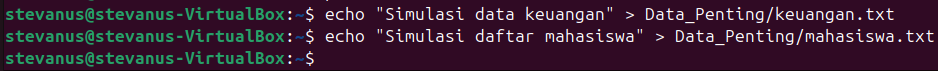
\includegraphics[width=0.75\textwidth]{Figure/04/gambar10.png}
	\caption{Proses penyiapan direktori dan data simulasi untuk target \textit{backup}.}
	\label{fig:m04-gambar10}
\end{figure}

\subsection{Sesi 1: Penulisan Skrip Bash Sederhana}
\label{sec:m04-sesi-1}

\begin{enumerate}
	\item Gunakan editor teks \texttt{nano} untuk membuat file berakhiran \texttt{.sh}.
	\begin{lstlisting}[language=bash, caption={Membuka editor nano}]
		$ nano script_backup.sh
	\end{lstlisting}
	
	\item Di dalam \textit{workspace nano}, ketikkan baris skrip di bawah ini. Jika sudah, simpan dengan menekan \texttt{Ctrl+O}, \texttt{Enter}, lalu \texttt{Ctrl+X} untuk menutup.
	\begin{lstlisting}[language=bash, caption={Struktur Skrip Automasi Backup Sederhana}]
		#!/bin/bash
		# Automasi proses duplikasi keamanan data
		
		SUMBER="Data_Penting"
		TUJUAN="Backup_$(date +%F)"
		
		echo "Sedang menyalin direktori: $SUMBER..."
		
		# Eksekusi proses copy rekursif ke variabel TUJUAN
		cp -r $SUMBER $TUJUAN
		
		echo "Proses backup selesai! Tersimpan di: $TUJUAN"
	\end{lstlisting}
\end{enumerate}

\begin{figure}[H]
	\centering
	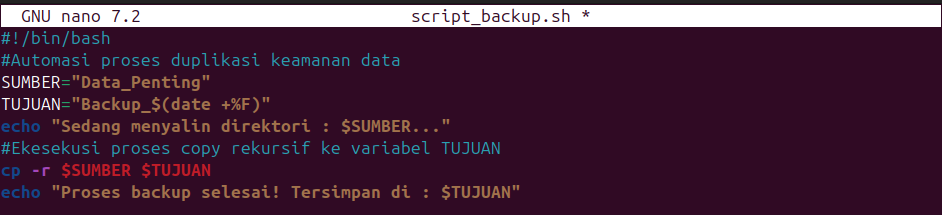
\includegraphics[width=0.75\textwidth]{Figure/04/gambar11.png}
	\caption{Tampilan penulisan skrip \textit{backup} memanfaatkan teks editor CLI terintegrasi.}
	\label{fig:m04-gambar11}
\end{figure}

\subsection{Sesi 2: Manipulasi Izin Execute dan Menjalankan Skrip}
\label{sec:m04-sesi-2}

\begin{enumerate}
	\item Berikan izin \textit{executable} pada file skrip. 
	\begin{lstlisting}[language=bash, caption={Memberikan izin eksekusi ke file script}]
		# Mengecek metadata dan izin file awal sebelum dimodifikasi
		$ ls -l script_backup.sh
		
		# Menambahkan modifier executable (+x)
		$ chmod +x script_backup.sh
		
		# Mengecek kembali, file akan berubah warna
		$ ls -l script_backup.sh
	\end{lstlisting}
	
	\item Panggil nama skrip tersebut dan verifikasi eksekusinya.
	\begin{lstlisting}[language=bash, caption={Eksekusi program bash}]
		# Menjalankan script di folder saat ini (./)
		$ ./script_backup.sh
		
		# Memeriksa hasil backup menggunakan perintah ls
		$ ls -l
	\end{lstlisting}
\end{enumerate}

\begin{figure}[H]
	\centering
	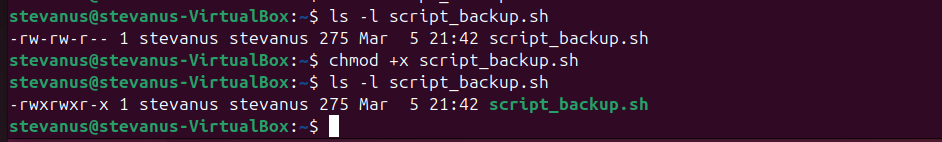
\includegraphics[width=0.75\textwidth]{Figure/04/gambar12.png}
	\caption{Validasi proses modifikasi izin eksekusi dan keberhasilan eksekusi automasi \textit{backup} pada terminal.}
	\label{fig:m04-gambar12}
\end{figure}

\newpage
\section{\textit{Hands On}}
\label{sec:m04-hands-on}

Pada bagian ini, setiap mahasiswa wajib mengerjakan tugas praktik mandiri yang mencakup materi pemahaman dari Modul 3 dan Modul 4 sebagai berikut:

\begin{enumerate}
	\item Buatlah struktur direktori berikut secara berurutan:
	\begin{itemize}
		\item Buat 2 direktori bernama \texttt{mahasiswa\_namaanda} dan \texttt{matakuliah\_namaanda}.
		\item Di dalam \texttt{mahasiswa\_namaanda}, buat file teks menggunakan \texttt{nano} bernama \texttt{datadiri\_namaanda.txt} yang berisi Nama, NIM, Prodi, dan Angkatan Anda.
		\item Di dalam \texttt{matakuliah\_namaanda}, buat file teks bernama \texttt{sistemoperasi\_namaanda.txt} yang memuat Nama, Kelas, dan Kode IF.
	\end{itemize}
	\item Pindahkan seluruh folder \texttt{matakuliah\_namaanda} ke dalam folder \texttt{mahasiswa\_namaanda} menggunakan perintah \texttt{mv}. Tampilkan isi file \texttt{sistemoperasi\_namaanda.txt} di terminal menggunakan \texttt{cat}.
	\item Demonstrasikan modifikasi hak akses dengan menghapus izin \textit{write} (\texttt{w}) pada file \texttt{datadiri\_namaanda.txt} menggunakan \texttt{chmod}.
	\item Susun sebuah \textit{shell script} (\texttt{backup\_tugas.sh}) yang akan mengotomatisasi penyalinan (\texttt{cp}) folder \texttt{mahasiswa\_namaanda} ke sebuah folder baru bernama \texttt{Arsip\_namaanda}.
	\item Berikan izin eksekusi (\texttt{chmod +x}) pada skrip tersebut dan jalankan skripnya di terminal. Verifikasi apakah folder arsip terbentuk dengan benar.
	\item Dokumentasikan setiap langkah dan perintah eksekusi terminal secara berurutan (wajib disertai \textit{screenshot}).
	\item Menyusun laporan praktikum sesuai \textit{template} resmi pada GitHub IF ITERA: \\
	\url{https://github.com/informatika-itera/IF25-12007-Sistem-Operasi/tree/main/Hands-On}
\end{enumerate}

Laporan \textbf{wajib} disusun menggunakan \LaTeX.